\documentclass{lab1-article}

\title{Rimbalzi di una pallina}

\usepackage{fancyvrb}
\usepackage{hyperref}
\makeatletter
\def\PY@reset{\let\PY@it=\relax \let\PY@bf=\relax%
    \let\PY@ul=\relax \let\PY@tc=\relax%
    \let\PY@bc=\relax \let\PY@ff=\relax}
\def\PY@tok#1{\csname PY@tok@#1\endcsname}
\def\PY@toks#1+{\ifx\relax#1\empty\else%
    \PY@tok{#1}\expandafter\PY@toks\fi}
\def\PY@do#1{\PY@bc{\PY@tc{\PY@ul{%
    \PY@it{\PY@bf{\PY@ff{#1}}}}}}}
\def\PY#1#2{\PY@reset\PY@toks#1+\relax+\PY@do{#2}}

\expandafter\def\csname PY@tok@gd\endcsname{\def\PY@tc##1{\textcolor[rgb]{0.63,0.00,0.00}{##1}}}
\expandafter\def\csname PY@tok@gu\endcsname{\let\PY@bf=\textbf\def\PY@tc##1{\textcolor[rgb]{0.50,0.00,0.50}{##1}}}
\expandafter\def\csname PY@tok@gt\endcsname{\def\PY@tc##1{\textcolor[rgb]{0.00,0.27,0.87}{##1}}}
\expandafter\def\csname PY@tok@gs\endcsname{\let\PY@bf=\textbf}
\expandafter\def\csname PY@tok@gr\endcsname{\def\PY@tc##1{\textcolor[rgb]{1.00,0.00,0.00}{##1}}}
\expandafter\def\csname PY@tok@cm\endcsname{\let\PY@it=\textit\def\PY@tc##1{\textcolor[rgb]{0.25,0.50,0.50}{##1}}}
\expandafter\def\csname PY@tok@vg\endcsname{\def\PY@tc##1{\textcolor[rgb]{0.10,0.09,0.49}{##1}}}
\expandafter\def\csname PY@tok@m\endcsname{\def\PY@tc##1{\textcolor[rgb]{0.40,0.40,0.40}{##1}}}
\expandafter\def\csname PY@tok@mh\endcsname{\def\PY@tc##1{\textcolor[rgb]{0.40,0.40,0.40}{##1}}}
\expandafter\def\csname PY@tok@go\endcsname{\def\PY@tc##1{\textcolor[rgb]{0.53,0.53,0.53}{##1}}}
\expandafter\def\csname PY@tok@ge\endcsname{\let\PY@it=\textit}
\expandafter\def\csname PY@tok@vc\endcsname{\def\PY@tc##1{\textcolor[rgb]{0.10,0.09,0.49}{##1}}}
\expandafter\def\csname PY@tok@il\endcsname{\def\PY@tc##1{\textcolor[rgb]{0.40,0.40,0.40}{##1}}}
\expandafter\def\csname PY@tok@cs\endcsname{\let\PY@it=\textit\def\PY@tc##1{\textcolor[rgb]{0.25,0.50,0.50}{##1}}}
\expandafter\def\csname PY@tok@cp\endcsname{\def\PY@tc##1{\textcolor[rgb]{0.74,0.48,0.00}{##1}}}
\expandafter\def\csname PY@tok@gi\endcsname{\def\PY@tc##1{\textcolor[rgb]{0.00,0.63,0.00}{##1}}}
\expandafter\def\csname PY@tok@gh\endcsname{\let\PY@bf=\textbf\def\PY@tc##1{\textcolor[rgb]{0.00,0.00,0.50}{##1}}}
\expandafter\def\csname PY@tok@ni\endcsname{\let\PY@bf=\textbf\def\PY@tc##1{\textcolor[rgb]{0.60,0.60,0.60}{##1}}}
\expandafter\def\csname PY@tok@nl\endcsname{\def\PY@tc##1{\textcolor[rgb]{0.63,0.63,0.00}{##1}}}
\expandafter\def\csname PY@tok@nn\endcsname{\let\PY@bf=\textbf\def\PY@tc##1{\textcolor[rgb]{0.00,0.00,1.00}{##1}}}
\expandafter\def\csname PY@tok@no\endcsname{\def\PY@tc##1{\textcolor[rgb]{0.53,0.00,0.00}{##1}}}
\expandafter\def\csname PY@tok@na\endcsname{\def\PY@tc##1{\textcolor[rgb]{0.49,0.56,0.16}{##1}}}
\expandafter\def\csname PY@tok@nb\endcsname{\def\PY@tc##1{\textcolor[rgb]{0.00,0.50,0.00}{##1}}}
\expandafter\def\csname PY@tok@nc\endcsname{\let\PY@bf=\textbf\def\PY@tc##1{\textcolor[rgb]{0.00,0.00,1.00}{##1}}}
\expandafter\def\csname PY@tok@nd\endcsname{\def\PY@tc##1{\textcolor[rgb]{0.67,0.13,1.00}{##1}}}
\expandafter\def\csname PY@tok@ne\endcsname{\let\PY@bf=\textbf\def\PY@tc##1{\textcolor[rgb]{0.82,0.25,0.23}{##1}}}
\expandafter\def\csname PY@tok@nf\endcsname{\def\PY@tc##1{\textcolor[rgb]{0.00,0.00,1.00}{##1}}}
\expandafter\def\csname PY@tok@si\endcsname{\let\PY@bf=\textbf\def\PY@tc##1{\textcolor[rgb]{0.73,0.40,0.53}{##1}}}
\expandafter\def\csname PY@tok@s2\endcsname{\def\PY@tc##1{\textcolor[rgb]{0.73,0.13,0.13}{##1}}}
\expandafter\def\csname PY@tok@vi\endcsname{\def\PY@tc##1{\textcolor[rgb]{0.10,0.09,0.49}{##1}}}
\expandafter\def\csname PY@tok@nt\endcsname{\let\PY@bf=\textbf\def\PY@tc##1{\textcolor[rgb]{0.00,0.50,0.00}{##1}}}
\expandafter\def\csname PY@tok@nv\endcsname{\def\PY@tc##1{\textcolor[rgb]{0.10,0.09,0.49}{##1}}}
\expandafter\def\csname PY@tok@s1\endcsname{\def\PY@tc##1{\textcolor[rgb]{0.73,0.13,0.13}{##1}}}
\expandafter\def\csname PY@tok@sh\endcsname{\def\PY@tc##1{\textcolor[rgb]{0.73,0.13,0.13}{##1}}}
\expandafter\def\csname PY@tok@sc\endcsname{\def\PY@tc##1{\textcolor[rgb]{0.73,0.13,0.13}{##1}}}
\expandafter\def\csname PY@tok@sx\endcsname{\def\PY@tc##1{\textcolor[rgb]{0.00,0.50,0.00}{##1}}}
\expandafter\def\csname PY@tok@bp\endcsname{\def\PY@tc##1{\textcolor[rgb]{0.00,0.50,0.00}{##1}}}
\expandafter\def\csname PY@tok@c1\endcsname{\let\PY@it=\textit\def\PY@tc##1{\textcolor[rgb]{0.25,0.50,0.50}{##1}}}
\expandafter\def\csname PY@tok@kc\endcsname{\let\PY@bf=\textbf\def\PY@tc##1{\textcolor[rgb]{0.00,0.50,0.00}{##1}}}
\expandafter\def\csname PY@tok@c\endcsname{\let\PY@it=\textit\def\PY@tc##1{\textcolor[rgb]{0.25,0.50,0.50}{##1}}}
\expandafter\def\csname PY@tok@mf\endcsname{\def\PY@tc##1{\textcolor[rgb]{0.40,0.40,0.40}{##1}}}
\expandafter\def\csname PY@tok@err\endcsname{\def\PY@bc##1{\setlength{\fboxsep}{0pt}\fcolorbox[rgb]{1.00,0.00,0.00}{1,1,1}{\strut ##1}}}
\expandafter\def\csname PY@tok@kd\endcsname{\let\PY@bf=\textbf\def\PY@tc##1{\textcolor[rgb]{0.00,0.50,0.00}{##1}}}
\expandafter\def\csname PY@tok@ss\endcsname{\def\PY@tc##1{\textcolor[rgb]{0.10,0.09,0.49}{##1}}}
\expandafter\def\csname PY@tok@sr\endcsname{\def\PY@tc##1{\textcolor[rgb]{0.73,0.40,0.53}{##1}}}
\expandafter\def\csname PY@tok@mo\endcsname{\def\PY@tc##1{\textcolor[rgb]{0.40,0.40,0.40}{##1}}}
\expandafter\def\csname PY@tok@kn\endcsname{\let\PY@bf=\textbf\def\PY@tc##1{\textcolor[rgb]{0.00,0.50,0.00}{##1}}}
\expandafter\def\csname PY@tok@mi\endcsname{\def\PY@tc##1{\textcolor[rgb]{0.40,0.40,0.40}{##1}}}
\expandafter\def\csname PY@tok@gp\endcsname{\let\PY@bf=\textbf\def\PY@tc##1{\textcolor[rgb]{0.00,0.00,0.50}{##1}}}
\expandafter\def\csname PY@tok@o\endcsname{\def\PY@tc##1{\textcolor[rgb]{0.40,0.40,0.40}{##1}}}
\expandafter\def\csname PY@tok@kr\endcsname{\let\PY@bf=\textbf\def\PY@tc##1{\textcolor[rgb]{0.00,0.50,0.00}{##1}}}
\expandafter\def\csname PY@tok@s\endcsname{\def\PY@tc##1{\textcolor[rgb]{0.73,0.13,0.13}{##1}}}
\expandafter\def\csname PY@tok@kp\endcsname{\def\PY@tc##1{\textcolor[rgb]{0.00,0.50,0.00}{##1}}}
\expandafter\def\csname PY@tok@w\endcsname{\def\PY@tc##1{\textcolor[rgb]{0.73,0.73,0.73}{##1}}}
\expandafter\def\csname PY@tok@kt\endcsname{\def\PY@tc##1{\textcolor[rgb]{0.69,0.00,0.25}{##1}}}
\expandafter\def\csname PY@tok@ow\endcsname{\let\PY@bf=\textbf\def\PY@tc##1{\textcolor[rgb]{0.67,0.13,1.00}{##1}}}
\expandafter\def\csname PY@tok@sb\endcsname{\def\PY@tc##1{\textcolor[rgb]{0.73,0.13,0.13}{##1}}}
\expandafter\def\csname PY@tok@k\endcsname{\let\PY@bf=\textbf\def\PY@tc##1{\textcolor[rgb]{0.00,0.50,0.00}{##1}}}
\expandafter\def\csname PY@tok@se\endcsname{\let\PY@bf=\textbf\def\PY@tc##1{\textcolor[rgb]{0.73,0.40,0.13}{##1}}}
\expandafter\def\csname PY@tok@sd\endcsname{\let\PY@it=\textit\def\PY@tc##1{\textcolor[rgb]{0.73,0.13,0.13}{##1}}}

\def\PYZbs{\char`\\}
\def\PYZus{\char`\_}
\def\PYZob{\char`\{}
\def\PYZcb{\char`\}}
\def\PYZca{\char`\^}
\def\PYZam{\char`\&}
\def\PYZlt{\char`\<}
\def\PYZgt{\char`\>}
\def\PYZsh{\char`\#}
\def\PYZpc{\char`\%}
\def\PYZdl{\char`\$}
\def\PYZhy{\char`\-}
\def\PYZsq{\char`\'}
\def\PYZdq{\char`\"}
\def\PYZti{\char`\~}
% for compatibility with earlier versions
\def\PYZat{@}
\def\PYZlb{[}
\def\PYZrb{]}
\makeatother


\begin{document}


\begin{article}
\selectlanguage{italian}

\maketitle

\secintro

Nel modello pi\`u semplice che possiamo formulare una pallina elastica che
rimbalza su una superficie rigida (e.g., il pavimento) perde una frazione $\gamma$
della sua energia indipendente dalla velocit\`a prima dell'impatto. Se lasciamo
cadere la pallina da un'altezza nota $h_0$, con velocit\`a iniziale nulla, sotto
l'azione della forza di gravit\`a, l'altezza massima raggiunta dopo $n$ rimbalzi
sar\`a dunque, sotto queste ipotesi:
\begin{align}\label{eq:modello}
  h_n = h_0 \gamma^n.
\end{align}

Lo scopo dell'esperienza \`e lo studio della dinamica dei rimbalzi di una
pallina elastica utilizzando lo smartphone per registrare il rumore prodotto dai
rimbalzi.

\secmaterialsdad

\begin{itemize}
\item Una pallina elastica.
\item Metro a nastro.
\item Smartphone o macchina fotografica digitale.
\end{itemize}


\secmeasurements

Misureremo i tempi dei vari rimbalzi attraverso l'analisi di una apposita
registrazione audio eseguita con lo smartphone. Come potete vedere nel
frammento di codice esemplificativo riportato nella pagine seguente,
un file audio in formato \emph{wave} pu\`o essere letto e trasformato in un
grafico---a questo punto si pu\`o lavorare con lo strumento zoom di matplotlib
ed il mouse per stimare i tempi.

\begin{figure}[!hb]
  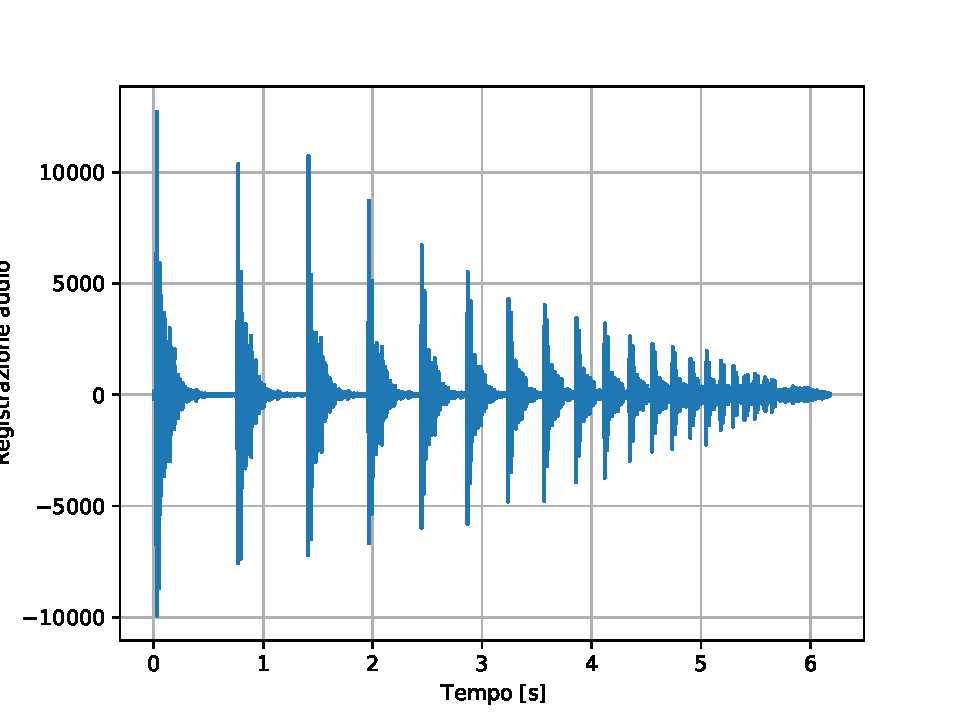
\includegraphics[width=\linewidth]{figures/rimbalzi_palla}
\end{figure}

\labsubsection{Analisi del file audio}

Analogamente a quanto fatto per l'esperienza della catenaria, misureremo
i tempi di rimbalzo manualmente utilizzando il \emph{mouse}. Notiamo che ogni
rimbalzo \`e caratterizzato da un \emph{attacco} estremamente rapido e da
una \emph{coda} relativamente pi\`u lunga. Si consiglia di eseguire uno
zoom stretto sui ciascun attacco per stimare con precisione il momento
dell'impatto; dovrete anche, va da s\'e, pensare a come stimare in modo
ragionevole l'incertezza associata.

(Man mano che la velocit\`a di impatto sul suolo diminuisce, anche la pressione
sonora si riduce, come si vede chiaramente dalla figura.)


\labsubsection{Stima dell'altezza massima}

\`E facile dimostrare che, nel nostro modello, l'altezza massima raggiunta tra
due rimbalzi successivi pu\`o essere stimata a partire dai tempi di rimbalzo
come
\begin{align}
  h_n = \frac{1}{8}g(t_n - t_{n-1})^2.
\end{align}
(Notiamo, per inciso, che questo non include un certo numero di effetti
potenzialmente rilevanti come la resistenza dell'aria.)

Realizzate un grafico dell'altezza $h_n$ in funzione dell'indice $n$ del rimbalzo.
Se il nostro modello descrive accuratamente i dati, questi ultimo dovrebbero
disporsi come un esponenziale (e quindi dovrebbero apparire come una retta
in scala semilogaritmica). Si fitti il grafico di dispersione con la~\eqref{eq:modello}
e si stimi il valore di $gamma$. Si confronti il valore di $h_0$ con la misura
diretta dell'altezza iniziale.


\secconsiderations

Avrete bisogno di un ambiente il pi\`u possibile silezioso per effettuare la
registrazione. Palline diverse perderanno una frazione diversa della loro energia
ad ogni rimbalzo, per cui si consiglia di fare un certo numero di prove per
trovare la configurazione ottimale (inclusa la misura dell'altezza iniziale da
cui la pallina viene fatta cadere).

Assicuratevi che la \emph{app} che utilizzate permetta di registrare in formato
\emph{wave}---possibilmente mono. Ce ne sono svariate per tutte le piattaforme.
Alternativamente avrete bisogno di un programma per convertire in formato
\emph{wave} il \emph{file} prodotto dal vostro smartphone (e.g., in \emph{mp3}).
\emph{Audacity}, reperibile da \url{https://www.audacityteam.org/}, \`e un
esempio di \emph{editor} audio \emph{open-source} e multipiattaforma, che
vi permette di fare la conversione (oltre ad un numero sconfinato di altre cose).


\onecolumn

\begin{Verbatim}[label=\makebox{\href{https://github.com/unipi-physics-labs/lab1-sheets/tree/main/snippy/dad_palla.py}{https://github.com/.../dad\_palla.py}},commandchars=\\\{\}]
\PY{k+kn}{import}\PY{+w}{ }\PY{n+nn}{wave}

\PY{k+kn}{import}\PY{+w}{ }\PY{n+nn}{numpy}\PY{+w}{ }\PY{k}{as}\PY{+w}{ }\PY{n+nn}{np}
\PY{k+kn}{from}\PY{+w}{ }\PY{n+nn}{matplotlib}\PY{+w}{ }\PY{k+kn}{import} \PY{n}{pyplot} \PY{k}{as} \PY{n}{plt}
\PY{k+kn}{from}\PY{+w}{ }\PY{n+nn}{scipy}\PY{n+nn}{.}\PY{n+nn}{optimize}\PY{+w}{ }\PY{k+kn}{import} \PY{n}{curve\PYZus{}fit}

\PY{n}{file\PYZus{}path} \PY{o}{=} \PY{l+s+s1}{\PYZsq{}}\PY{l+s+s1}{macro/data/bouncing\PYZus{}ball3.wav}\PY{l+s+s1}{\PYZsq{}}
\PY{c+c1}{\PYZsh{} Apertura del file audio, vedi https://docs.python.org/3/library/wave.html}
\PY{n}{stream} \PY{o}{=} \PY{n}{wave}\PY{o}{.}\PY{n}{open}\PY{p}{(}\PY{n}{file\PYZus{}path}\PY{p}{)}
\PY{n}{signal} \PY{o}{=} \PY{n}{np}\PY{o}{.}\PY{n}{frombuffer}\PY{p}{(}\PY{n}{stream}\PY{o}{.}\PY{n}{readframes}\PY{p}{(}\PY{n}{stream}\PY{o}{.}\PY{n}{getnframes}\PY{p}{(}\PY{p}{)}\PY{p}{)}\PY{p}{,} \PY{n}{dtype}\PY{o}{=}\PY{n}{np}\PY{o}{.}\PY{n}{int16}\PY{p}{)}
\PY{c+c1}{\PYZsh{} Importante: se il file originale e` stereo dobbiamo prendere solo uno dei canali.}
\PY{k}{if} \PY{n}{stream}\PY{o}{.}\PY{n}{getnchannels}\PY{p}{(}\PY{p}{)} \PY{o}{==} \PY{l+m+mi}{2}\PY{p}{:}
    \PY{n}{signal} \PY{o}{=} \PY{n}{signal}\PY{p}{[}\PY{p}{:}\PY{p}{:}\PY{l+m+mi}{2}\PY{p}{]}
\PY{c+c1}{\PYZsh{} L\PYZsq{}unica cosa che ci manca e` l\PYZsq{}array dei tempi corrispondenti ai singoli campioni.}
\PY{n}{t} \PY{o}{=} \PY{n}{np}\PY{o}{.}\PY{n}{arange}\PY{p}{(}\PY{n+nb}{len}\PY{p}{(}\PY{n}{signal}\PY{p}{)}\PY{p}{)} \PY{o}{/} \PY{n}{stream}\PY{o}{.}\PY{n}{getframerate}\PY{p}{(}\PY{p}{)}

\PY{c+c1}{\PYZsh{} A questo punto siamo pronti per analizzare il tracciato audio. Una volta}
\PY{c+c1}{\PYZsh{} messi i dati in un grafico di matplotlib possiamo utilizzare lo strumento}
\PY{c+c1}{\PYZsh{} zoom ed il mouse per misurare i tempi di rimbalzo della pallina.}
\PY{n}{plt}\PY{o}{.}\PY{n}{figure}\PY{p}{(}\PY{l+s+s1}{\PYZsq{}}\PY{l+s+s1}{Rimbalzi pallina}\PY{l+s+s1}{\PYZsq{}}\PY{p}{)}
\PY{n}{plt}\PY{o}{.}\PY{n}{plot}\PY{p}{(}\PY{n}{t}\PY{p}{,} \PY{n}{signal}\PY{p}{)}
\PY{n}{plt}\PY{o}{.}\PY{n}{xlabel}\PY{p}{(}\PY{l+s+s1}{\PYZsq{}}\PY{l+s+s1}{Tempo [s]}\PY{l+s+s1}{\PYZsq{}}\PY{p}{)}
\PY{n}{plt}\PY{o}{.}\PY{n}{savefig}\PY{p}{(}\PY{l+s+s1}{\PYZsq{}}\PY{l+s+s1}{audio\PYZus{}rimbalzi.pdf}\PY{l+s+s1}{\PYZsq{}}\PY{p}{)}

\PY{c+c1}{\PYZsh{} Supponiamo di aver preso a mano questa serie di tempi di rimbalzo.}
\PY{n}{t} \PY{o}{=} \PY{p}{[}\PY{l+m+mf}{0.01961451}\PY{p}{,} \PY{l+m+mf}{0.69562358}\PY{p}{,} \PY{l+m+mf}{1.23981859}\PY{p}{,} \PY{l+m+mf}{1.679161}\PY{p}{,} \PY{l+m+mf}{2.04113379}\PY{p}{,} \PY{l+m+mf}{2.33979592}\PY{p}{]}
\PY{c+c1}{\PYZsh{} Cercate di stimare ragionevolmente gli errori...}
\PY{n}{sigma\PYZus{}t} \PY{o}{=} \PY{l+m+mf}{0.005}
\PY{c+c1}{\PYZsh{} Calcolo delle differenze di tempo.}
\PY{n}{dt} \PY{o}{=} \PY{n}{np}\PY{o}{.}\PY{n}{diff}\PY{p}{(}\PY{n}{t}\PY{p}{)}
\PY{c+c1}{\PYZsh{} Creazione dell\PYZsq{}array con gli indici dei rimbalzi.}
\PY{n}{n} \PY{o}{=} \PY{n}{np}\PY{o}{.}\PY{n}{arange}\PY{p}{(}\PY{n+nb}{len}\PY{p}{(}\PY{n}{dt}\PY{p}{)}\PY{p}{)} \PY{o}{+} \PY{l+m+mf}{1.}
\PY{c+c1}{\PYZsh{} Calcolo dell\PYZsq{}altezza massima e propagazione degli errori.}
\PY{n}{h} \PY{o}{=} \PY{l+m+mf}{9.81} \PY{o}{*} \PY{p}{(}\PY{n}{dt}\PY{o}{*}\PY{o}{*}\PY{l+m+mf}{2.}\PY{p}{)} \PY{o}{/} \PY{l+m+mf}{8.0}
\PY{n}{dh} \PY{o}{=} \PY{l+m+mf}{2.0} \PY{o}{*} \PY{n}{np}\PY{o}{.}\PY{n}{sqrt}\PY{p}{(}\PY{l+m+mf}{2.0}\PY{p}{)} \PY{o}{*} \PY{n}{h} \PY{o}{*} \PY{n}{sigma\PYZus{}t} \PY{o}{/} \PY{n}{dt}

\PY{k}{def}\PY{+w}{ }\PY{n+nf}{expo}\PY{p}{(}\PY{n}{n}\PY{p}{,} \PY{n}{h0}\PY{p}{,} \PY{n}{gamma}\PY{p}{)}\PY{p}{:}
\PY{+w}{    }\PY{l+s+sd}{\PYZdq{}\PYZdq{}\PYZdq{}Modello di fit.}
\PY{l+s+sd}{    \PYZdq{}\PYZdq{}\PYZdq{}}
    \PY{k}{return} \PY{n}{h0} \PY{o}{*} \PY{n}{gamma}\PY{o}{*}\PY{o}{*}\PY{n}{n}

\PY{n}{plt}\PY{o}{.}\PY{n}{figure}\PY{p}{(}\PY{l+s+s1}{\PYZsq{}}\PY{l+s+s1}{Altezza dei rimbalzi}\PY{l+s+s1}{\PYZsq{}}\PY{p}{)}
\PY{n}{plt}\PY{o}{.}\PY{n}{errorbar}\PY{p}{(}\PY{n}{n}\PY{p}{,} \PY{n}{h}\PY{p}{,} \PY{n}{dh}\PY{p}{,} \PY{n}{fmt}\PY{o}{=}\PY{l+s+s1}{\PYZsq{}}\PY{l+s+s1}{o}\PY{l+s+s1}{\PYZsq{}}\PY{p}{)}
\PY{n}{popt}\PY{p}{,} \PY{n}{pcov} \PY{o}{=} \PY{n}{curve\PYZus{}fit}\PY{p}{(}\PY{n}{expo}\PY{p}{,} \PY{n}{n}\PY{p}{,} \PY{n}{h}\PY{p}{,} \PY{n}{sigma}\PY{o}{=}\PY{n}{dh}\PY{p}{)}
\PY{n}{h0\PYZus{}hat}\PY{p}{,} \PY{n}{gamma\PYZus{}hat} \PY{o}{=} \PY{n}{popt}
\PY{n}{sigma\PYZus{}h0}\PY{p}{,} \PY{n}{sigma\PYZus{}gamma} \PY{o}{=} \PY{n}{np}\PY{o}{.}\PY{n}{sqrt}\PY{p}{(}\PY{n}{pcov}\PY{o}{.}\PY{n}{diagonal}\PY{p}{(}\PY{p}{)}\PY{p}{)}
\PY{n+nb}{print}\PY{p}{(}\PY{n}{h0\PYZus{}hat}\PY{p}{,} \PY{n}{sigma\PYZus{}h0}\PY{p}{,} \PY{n}{gamma\PYZus{}hat}\PY{p}{,} \PY{n}{sigma\PYZus{}gamma}\PY{p}{)}
\PY{n}{x} \PY{o}{=} \PY{n}{np}\PY{o}{.}\PY{n}{linspace}\PY{p}{(}\PY{l+m+mf}{0.0}\PY{p}{,} \PY{l+m+mf}{6.0}\PY{p}{,} \PY{l+m+mi}{100}\PY{p}{)}
\PY{n}{plt}\PY{o}{.}\PY{n}{plot}\PY{p}{(}\PY{n}{x}\PY{p}{,} \PY{n}{expo}\PY{p}{(}\PY{n}{x}\PY{p}{,} \PY{n}{h0\PYZus{}hat}\PY{p}{,} \PY{n}{gamma\PYZus{}hat}\PY{p}{)}\PY{p}{)}
\PY{n}{plt}\PY{o}{.}\PY{n}{yscale}\PY{p}{(}\PY{l+s+s1}{\PYZsq{}}\PY{l+s+s1}{log}\PY{l+s+s1}{\PYZsq{}}\PY{p}{)}
\PY{n}{plt}\PY{o}{.}\PY{n}{grid}\PY{p}{(}\PY{n}{which}\PY{o}{=}\PY{l+s+s1}{\PYZsq{}}\PY{l+s+s1}{both}\PY{l+s+s1}{\PYZsq{}}\PY{p}{,} \PY{n}{ls}\PY{o}{=}\PY{l+s+s1}{\PYZsq{}}\PY{l+s+s1}{dashed}\PY{l+s+s1}{\PYZsq{}}\PY{p}{,} \PY{n}{color}\PY{o}{=}\PY{l+s+s1}{\PYZsq{}}\PY{l+s+s1}{gray}\PY{l+s+s1}{\PYZsq{}}\PY{p}{)}
\PY{n}{plt}\PY{o}{.}\PY{n}{xlabel}\PY{p}{(}\PY{l+s+s1}{\PYZsq{}}\PY{l+s+s1}{Rimbalzo}\PY{l+s+s1}{\PYZsq{}}\PY{p}{)}
\PY{n}{plt}\PY{o}{.}\PY{n}{ylabel}\PY{p}{(}\PY{l+s+s1}{\PYZsq{}}\PY{l+s+s1}{Altezza massima [m]}\PY{l+s+s1}{\PYZsq{}}\PY{p}{)}
\PY{n}{plt}\PY{o}{.}\PY{n}{savefig}\PY{p}{(}\PY{l+s+s1}{\PYZsq{}}\PY{l+s+s1}{altezza\PYZus{}rimbalzi.pdf}\PY{l+s+s1}{\PYZsq{}}\PY{p}{)}

\PY{n}{plt}\PY{o}{.}\PY{n}{show}\PY{p}{(}\PY{p}{)}
\end{Verbatim}



\end{article}
\end{document}
